\documentclass{beamer}
\usetheme{Wrexham}  
\usepackage{graphicx}

\usepackage{caption}
\usepackage{subcaption}
 
\begin{document}
\title{Compressed Sensing as a tool for Video Analysis}
\subtitle{}
\author{Rhian Davies}

\date{\today}

\begin{frame}[plain] 
  \titlepage
\end{frame}



\begin{frame}
  \frametitle{Topics of interest}
  \begin{itemize}
  \item Detection and tracking of foreground in video
  \item Automatic detection of anomalous behaviour
  \item The sensing and compressing of signals 
  \end{itemize}

\end{frame}

\begin{frame}
  \frametitle{Analysing images mathmatically}

  \begin{itemize}
%  \item Assume images are black and white.
  \item An image is a matrix of pixels, with each pixel being represented by a number. 
\item This number is the grayscale intensity or luminance.
  \end{itemize}
  \begin{figure}[h]
\label{fig:grayscale}
    \centering
    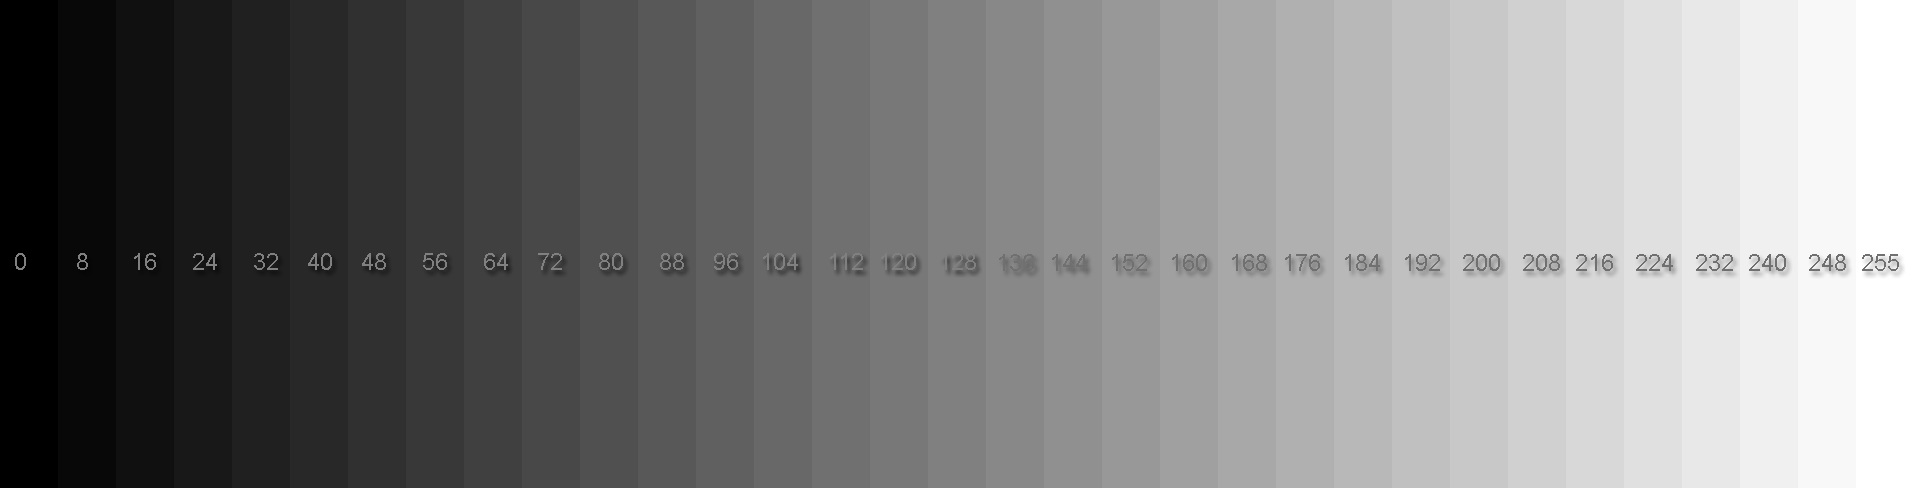
\includegraphics[height=2cm]{grayscale}
  %  \caption{Grayscale intensity}
    \end{figure}

\begin{figure}[h]
  \centering
  \[X_t =    \left( \begin{array}{ccc}
54 & 106 & 69 \\
220 & 7 & 3 \\
6 & 45 & 101 \end{array} \right)\] 
\end{figure}


 \begin{equation*}
    \label{eq:3}
X_t = [54,106,69,220,7,3,6,45,101]  \quad t= 1:T  
  \end{equation*}
\end{frame}

\begin{frame}
  \frametitle{Example}
Imagine you take a high quality picture and you wish to share this on the internet. If you used the full image uploading and viewing would take a long time. 

JPEG2000 compresses the image and but still retains the essential features of your image.

\begin{figure}
        \centering
        \begin{subfigure}[b]{0.4\textwidth}
                \centering
                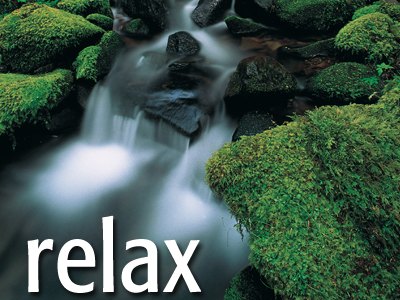
\includegraphics[width=\textwidth]{relax1}
                \caption{Original image}
                \label{fig:gull}
        \end{subfigure}
        \begin{subfigure}[b]{0.4\textwidth}
                \centering
                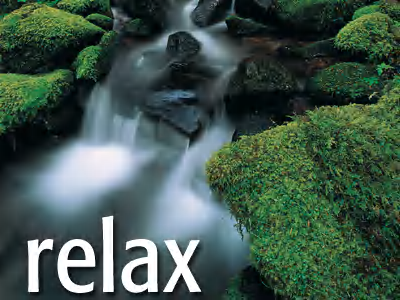
\includegraphics[width=\textwidth]{relax2}
                \caption{JPEG2000 compression}
                \label{fig:tiger}
        \end{subfigure}

\end{figure}

\end{frame}

%\begin{frame}
%  \frametitle{Nyquist – Shannon sampling theorem}

%If a function $X_t$ contains no frequencies higher than $N$ hertz, it is completely determined by giving its ordinates at a series of points spaced $\frac{1}{2N}$ seconds apart.

%Want to double your resolution? Double the number of pixels.
%\end{frame}


\begin{frame}
  \frametitle{Spasity and wavelet transformation}
Achievable resolution is dependant on the information content of the image. If an image has low information content  it is said to be sparse and can be perfectly recostructed from a small number of measurements. 

\bf{Nearly all real world images exhibit this sparsity property when transformed using a wavelet basis.}

  \begin{figure}[h]
    \centering
    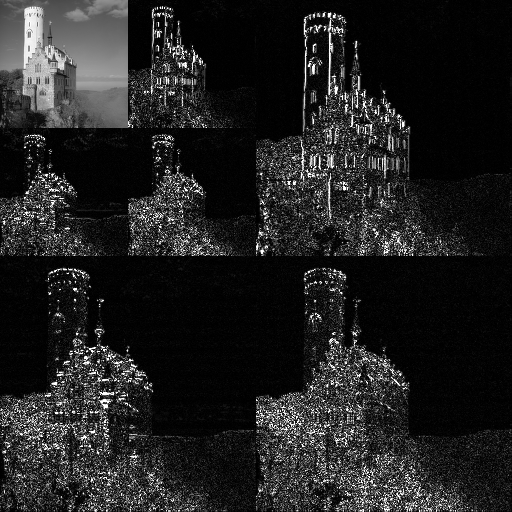
\includegraphics[height = 4cm]{wavelets}
    \caption{Wavelet transform}
    \label{fig:wavelet}
  \end{figure}

Note that most of the pixels here are black indicating low information content.
 \end{frame}

\begin{frame}
  \frametitle{Sparsity and CS}
  Let a signal be represented by $x$, of length $N$ and assume that the signal is $K$- sparse.

  \begin{equation}
    \label{eq:2}
    y = \phi x
  \end{equation}
Take a sample $y$ of size $M$ of the signal according to some measurement matrix $\phi$. ( $M < < N$.) 
We can use this $y$ to transmit the signal (e.g over the internet) or use it to perform video analysis such as determining if the pixel belongs to the foreground of a video.

How do we get back to $x$?
\end{frame}

\begin{frame}
  \frametitle{Reconstruction}
Linear algebra tells us that equation \ref{eq:1} is an underdetermined system  and that there is exists no unique solution. But, if we know that $x$  is $K$-sparse we can reconstuct the signal well.

\begin{equation}
  \label{eq:1}
  y = \phi x
\end{equation}

Possible methods include $l_1$ minimization and basis pursuit.

What effects do different reconstruction algorithms have on the computation time and final quality of the reconstruction?
\end{frame}

\begin{frame}
  \begin{figure}[h]
    \centering
    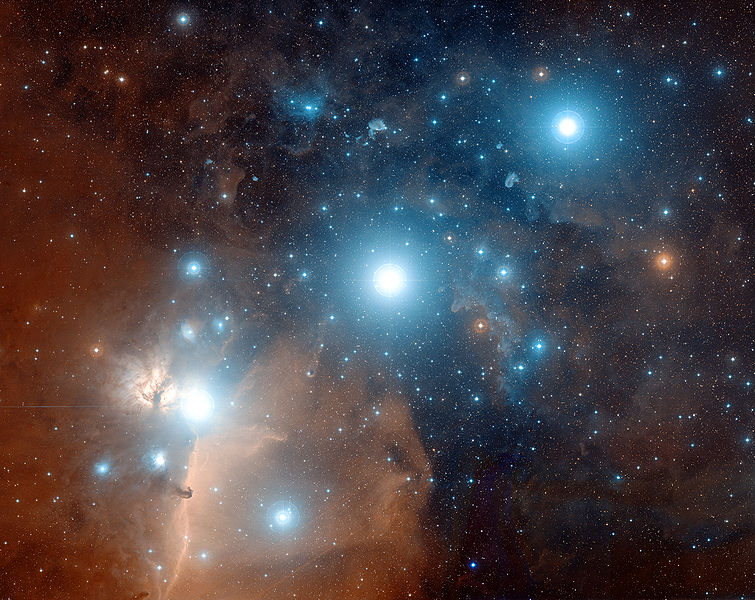
\includegraphics[height=6cm]{astrophotography}
    \caption{Astrophotography}
    \label{fig:astro}
  \end{figure}
\end{frame}
 
  \begin{frame}
    \begin{figure}[h]
  \centering
  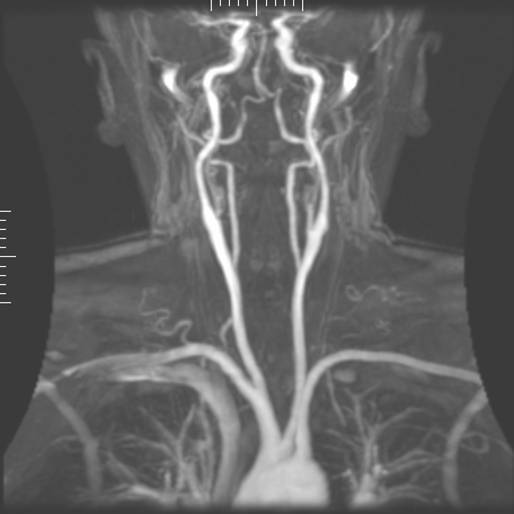
\includegraphics[height=6cm]{mri}
  \caption{MRI }
  \label{fig:mri}
\end{figure}
  \end{frame}

  \begin{frame}
  \begin{figure}[h]
  \centering
  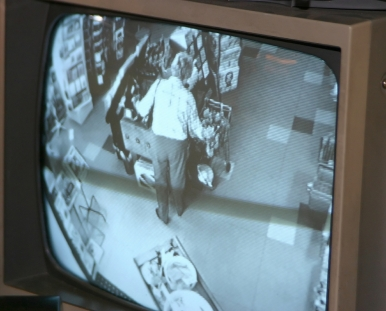
\includegraphics[height=6cm]{cctv}
  \caption{Analysing CCTV footage}
  \label{fig:cctv}
\end{figure}  
  \end{frame}


 \end{document}


